\RequirePackage{fix-cm}
\documentclass[12pt,letterpaper]{article}
\usepackage[margin=1in,headheight=15pt,headsep=15pt]{geometry}
\usepackage{amsmath,amssymb,graphicx,booktabs,array,float,fancyhdr,lastpage,hyperref}
\usepackage{microtype,needspace,fontspec,placeins,indentfirst}
\usepackage[UTF8,fontset=none,scheme=plain]{ctex}
\setmainfont{Times New Roman}
\setCJKmainfont{SimSun}[BoldFont=SimHei,ItalicFont=KaiTi,BoldItalicFont=KaiTi]
\setCJKsansfont{SimHei}
\setCJKmonofont{SimSun}
\ctexset{figurename=图,tablename=表}
\setlength{\parindent}{2em}
\setlength{\parskip}{0pt}
\setlength{\emergencystretch}{3em}
\hypersetup{hidelinks,pdftitle={第五章灵敏性分析：语言修改审阅稿}}
\pagestyle{fancy}\fancyhf{}
\fancyhead[L]{\small 第五章：灵敏性分析}
\fancyhead[R]{\small 语言修改审阅稿}
\fancyfoot[C]{\small 第 \thepage\ 页，共 \pageref{LastPage} 页}
\renewcommand{\headrulewidth}{0.4pt}
\graphicspath{{../../results/chapter5_review/fig13/}{../../results/sensitivity_linear/figures/}}
\renewcommand{\topfraction}{0.95}
\renewcommand{\bottomfraction}{0.9}
\renewcommand{\textfraction}{0.05}
\renewcommand{\floatpagefraction}{0.65}
\raggedbottom
\clubpenalty=10000
\widowpenalty=10000
\displaywidowpenalty=10000
\begin{document}
\setcounter{section}{4}
\setcounter{table}{3}
\setcounter{figure}{10}
\section{灵敏性分析}

本章以题目给定的三个早期位置为输入，分析初始运动、气动参数和空气密度对球门交点及到达时间的影响。计算采用重力、阻力和马格努斯力模型，空气保持静止，自旋保持恒定，足球质量固定为 0.43 kg，半径固定为 0.11 m。


\begin{table}[H]
\centering
\small
\renewcommand{\arraystretch}{1.16}
\caption{题给算例的早期位置}
\begin{tabular}{lccc}
\toprule
时间 $t$（s） & $x$（m） & $y$（m） & $z$（m）\\
\midrule
0 & 0 & 0 & 0.11\\
0.05 & 1.50 & 0.45 & 0.44\\
0.10 & 2.96 & 0.86 & 0.74\\
\bottomrule
\end{tabular}
\end{table}

按照第四章的反演方法，以 30 rad/s 为自旋参考模长，得到初始状态


\begin{equation*}
\begin{aligned}
\boldsymbol v_0&=(30.3784,\ 9.4074,\ 6.8974)\ \mathrm{m/s},\\
\boldsymbol\omega_0&=(19.7434,\ 1.2060,\ -22.5553)\ \mathrm{rad/s}.
\end{aligned}
\end{equation*}

相应的阻力系数为 $C_D=0.3623$，线性升力参数为 $\alpha=2.2877$，早期最大坐标残差为 0.784 mm。该轨迹在 $t_g^*=0.398967$ s 到达球门平面，交点为 $(y_g^*,z_g^*)=(2.6159,1.9526)$ m。


以下以该轨迹为基准，先逐项改变参数，识别各因素对交点和到达时间的影响；再保持早期位置约束，考察不同参数组合产生的预测差异；最后通过多参数联合扰动，求得交点分布及其统计范围。


\FloatBarrier
\subsection{单参数对交点和到达时间的影响}

每次改变一项参数，其余参数保持基准值。九项参数的扫描范围见表 5；百分比表示相对基准值的变化，方向角以基准方向为中心增减。每项参数取 41 个等间隔值，共计算 369 条轨迹。

\begin{table}[H]\centering\small
\renewcommand{\arraystretch}{1.15}
\caption{九项参数的扫描范围}
\begin{tabular}{lc}\toprule
参数 & 扰动范围\\\midrule
初速度大小 & $\pm$5\%\\
初速度水平角 & $\pm$$2^\circ$\\
初速度仰角 & $\pm$$2^\circ$\\
自旋大小 & $\pm$10\%\\
旋转轴方位角 & $\pm$$2^\circ$\\
旋转轴仰角 & $\pm$$2^\circ$\\
阻力系数 & $\pm$10\%\\
升力参数 & $\pm$10\%\\
空气密度 & $\pm$10\%\\
\bottomrule\end{tabular}\end{table}


\Needspace{5\baselineskip}
以交点和到达时间相对基准轨迹的变化衡量参数影响，定义


\begin{equation*}
\begin{aligned}
\Delta y_g&=y_g-y_g^*,\qquad
\Delta z_g=z_g-z_g^*,\qquad
\Delta t_g=t_g-t_g^*,\\
D_g&=\sqrt{(\Delta y_g)^2+(\Delta z_g)^2}.
\end{aligned}
\end{equation*}

图 11、图 12 分别展示九项参数的交点响应和到达时间响应。表 6 从扫描结果中取方向角的 $\pm$$1^\circ$ 扰动和其余参数的 $\pm$5\% 扰动，列出正、负两次变化中较大的交点位移与到达时间变化。


\begin{table}[H]
\centering
\small
\renewcommand{\arraystretch}{1.16}
\caption{单参数扰动对球门交点和到达时间的影响}
\begin{tabular}{lccc}
\toprule
参数 & 比较扰动 & 最大 $D_g$（cm） & 最大 $\lvert\Delta t_g\rvert$（ms）\\
\midrule
初速度大小 & $\pm$5\% & 8.356 & 20.659\\
初速度水平角 & $\pm$$1^\circ$ & 20.070 & 1.965\\
初速度仰角 & $\pm$$1^\circ$ & 20.218 & 1.692\\
自旋大小 & $\pm$5\% & 3.873 & 0.287\\
旋转轴方位角 & $\pm$$1^\circ$ & 1.002 & 0.071\\
旋转轴仰角 & $\pm$$1^\circ$ & 0.852 & 0.084\\
阻力系数 & $\pm$5\% & 0.620 & 2.274\\
升力参数 & $\pm$5\% & 3.873 & 0.287\\
空气密度 & $\pm$5\% & 4.142 & 1.990\\
\bottomrule
\end{tabular}
\end{table}

在表 6 的比较幅度下，初速度方向的变化主要体现在交点位置上：水平角或仰角改变 $1^\circ$，交点移动约 0.20 m。球速的变化则显著影响到达时间，$\pm$5\% 的扰动使到达时间最多改变 20.659 ms，同时产生最大 8.356 cm 的交点位移。这是因为速度方向直接决定横向和竖直运动，而球速改变了足球到达球门所需的时间，从而改变重力和气动力累积作用的结果。


自旋大小和升力参数的响应曲线重合，源于线性马格努斯力中二者的乘积关系：$\boldsymbol F_L$ 与 $\alpha\boldsymbol\omega$ 成正比。分别将自旋大小或 $\alpha$ 改变相同比例，会产生相同的力和轨迹变化；若二者按相反比例调整，则有


\begin{equation*}
\boldsymbol\omega_0'=k\boldsymbol\omega_0,\qquad
\alpha'=\alpha/k
\quad\Longrightarrow\quad
\boldsymbol F_L'=\boldsymbol F_L,\qquad k>0.
\end{equation*}

因此，不同的自旋大小与升力参数可以对应相同的轨迹。旋转轴方向则通过改变 $\boldsymbol\omega\times\boldsymbol v$ 影响偏转方向和大小。空气密度同时缩放阻力与马格努斯力，因而其变化会共同影响减速和弯曲过程。


\begin{figure}[!htbp]
\centering
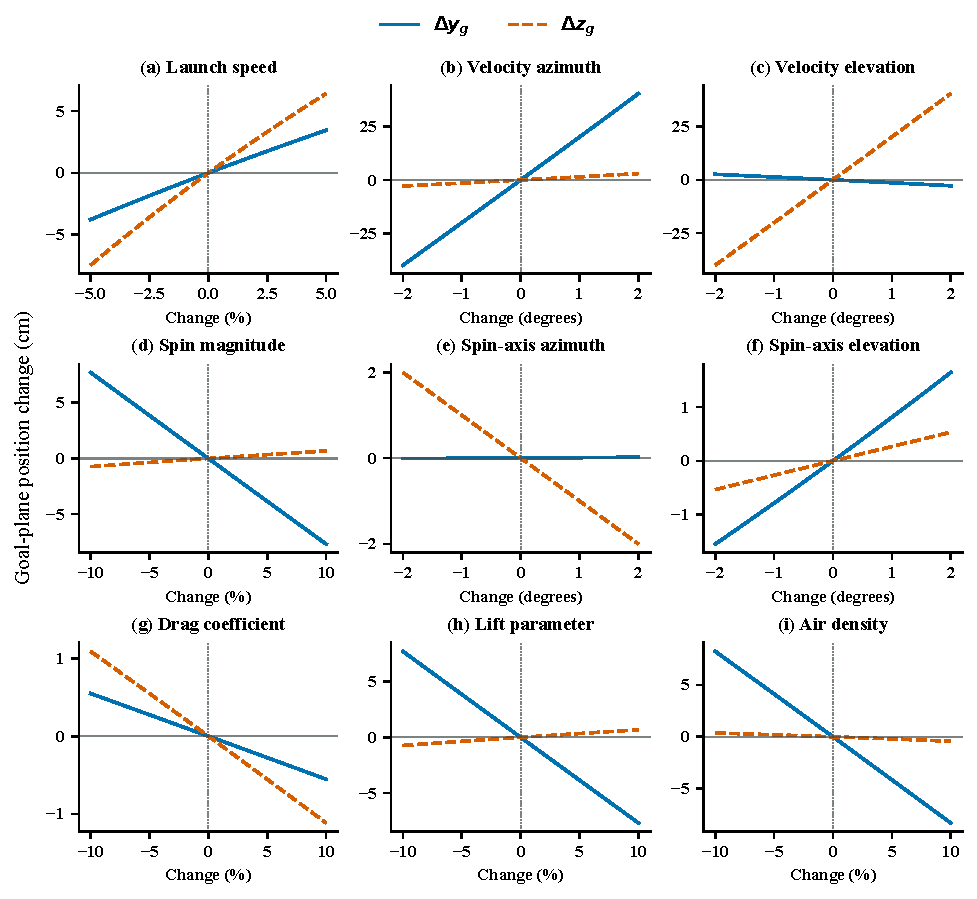
\includegraphics[clip,width=\textwidth]{one_factor_position_response.pdf}
\caption{九项单参数的球门位置响应。蓝色实线表示横向变化 $\Delta y_g$，橙色虚线表示高度变化 $\Delta z_g$，单位为 cm。各子图纵轴分别定标。}
\end{figure}


\begin{figure}[!htbp]
\centering
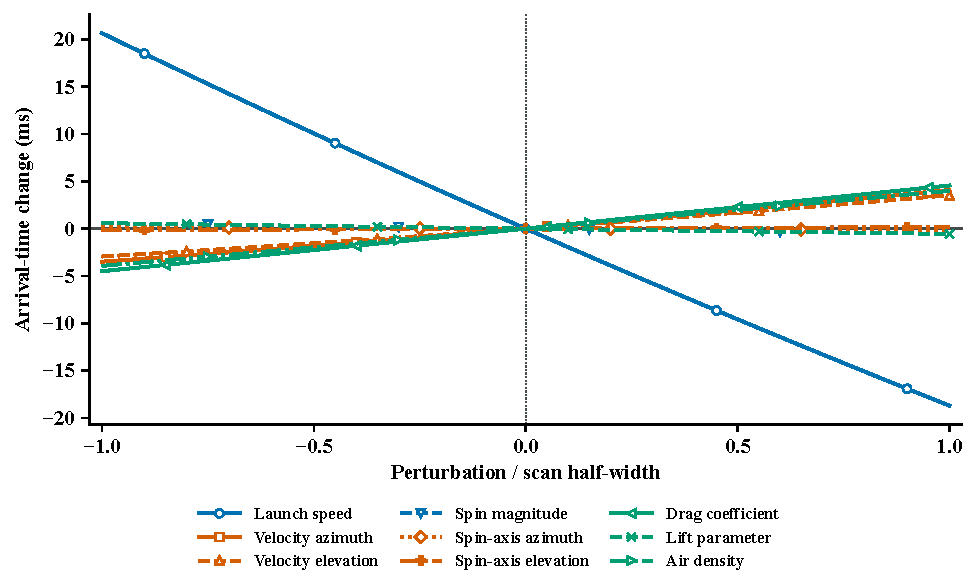
\includegraphics[clip,width=\textwidth]{one_factor_time_response.pdf}
\caption{九项单参数的到达时间响应。横轴为扰动量与扫描半宽之比，$\pm1$ 对应各参数的扫描端点；纵轴为 $\Delta t_g$（ms），正值表示晚到。}
\end{figure}


\FloatBarrier
\subsection{早期位置约束下的预测差异}

上一节在其余参数固定时考察单项变化。本节进一步考察：当不同参数组合都能近似重现同一组早期位置时，后续球门交点会相差多少。


以第四章的气动参考值 $C_D^*$ 和 $\alpha^*$ 为尺度，定义


\begin{equation*}
\lambda_D=C_D/C_D^*,\qquad
\lambda_\alpha=\alpha/\alpha^*.
\end{equation*}

两个系数倍数分别在 $[1.2,1.8]$ 内取 17 个等间隔值，形成 $17\times17$ 个组合。对每个组合，将初始自旋分量 $\omega_{x0}$ 在 $[-60,60]$ rad/s 内取 33 个等间隔值，再拟合三个初速度分量及其余两个自旋分量，使轨迹匹配表 4 的早期位置。搜索中总速度不超过 35 m/s，各自旋分量的绝对值不超过 60 rad/s，并以最大早期坐标残差不超过 2 mm 为约束条件。


补充搜索在 153 个气动参数组合下得到 5049 条满足约束的轨迹。其中，将两个系数倍数的范围收窄到 $[1.35,1.65]$，即两项气动参数在基准值附近各变化 $\pm$10\%，相应得到 63 个参数组合、2079 条轨迹。对应的交点与到达时间范围见表 7，交点分布见图 13。


\begin{table}[H]
\centering
\small
\renewcommand{\arraystretch}{1.16}
\caption{早期位置约束下的球门交点范围}
\begin{tabular}{lccc}
\toprule
两个系数倍数的范围 & $y_g$（m） & $z_g$（m） & $t_g$（s）\\
\midrule
$[1.35,1.65]$ & 2.5538--2.6550 & 1.9061--2.0369 & 0.3972--0.4025\\
$[1.2,1.8]$ & 2.5478--2.6601 & 1.8972--2.0430 & 0.3972--0.4043\\
\bottomrule
\end{tabular}
\end{table}

\Needspace{5\baselineskip}

在较宽的参数范围内，所搜索轨迹的球门交点相对基准轨迹最大偏移 0.1074 m。每组气动参数的最小残差解集中在自旋分量边界，单独绘制这些解会形成两簇；满足 2 mm 位置约束的中间自旋状态则形成连接两簇的交点带，如图 13 所示。这表明，初始速度与自旋可以补偿气动参数对短时位置的影响，而不同受力过程在后续飞行中累积，形成交点差异。


\begin{figure}[!htbp]
\centering
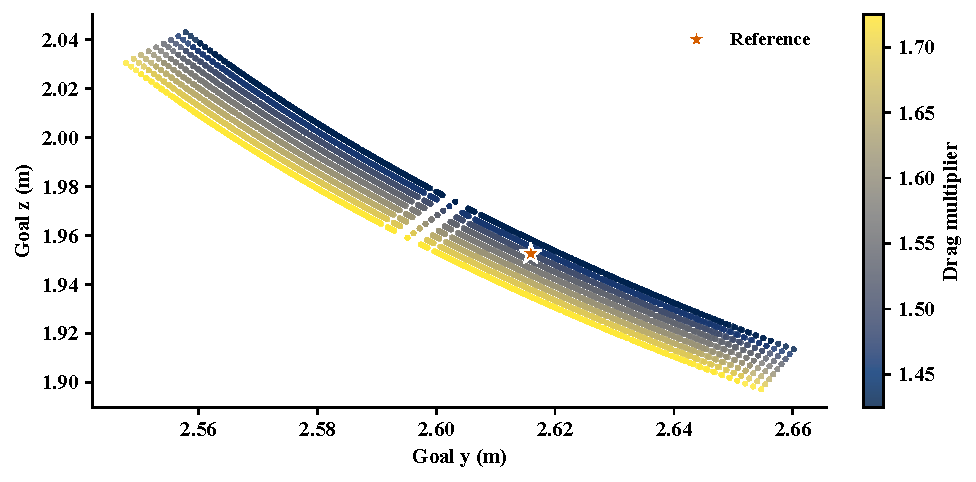
\includegraphics[clip,width=.88\textwidth]{conditional_crossings_review.pdf}
\caption{2 mm 早期位置约束下补充搜索得到的 5049 个交点。颜色表示 $\lambda_D$，橙色星号为基准轨迹。}
\end{figure}


\FloatBarrier
\subsection{联合扰动下的交点分布}

为考察多项条件同时变化的结果，在第 5.1 节的扫描范围内独立均匀抽取九项参数，生成 100000 组输入。质量、半径和初始位置保持不变，将各组输入代入运动方程，计算发射条件与气动参数共同变化产生的交点分布。


\begin{table}[H]
\centering
\small
\renewcommand{\arraystretch}{1.16}
\caption{十万条联合扰动轨迹的交点与到达时间}
\begin{tabular}{lcc}
\toprule
输出量 & 样本最小值--最大值 & 单坐标中心 95\% 区间\\
\midrule
$y_g$（m） & 1.9633--3.2143 & 2.1858--3.0505\\
$z_g$（m） & 1.4381--2.4646 & 1.5534--2.3535\\
$t_g$（s） & 0.3685--0.4346 & 0.3783--0.4218\\
\bottomrule
\end{tabular}
\end{table}

表 8 中的中心 95\% 区间由各输出的 2.5\% 和 97.5\% 分位数确定。模拟交点的均值为 $(2.6170,1.9511)$ m，横向和高度标准差分别为 0.2455 m、0.2360 m；相对基准交点的最大位移为 0.801 m。


为同时描述横向和高度的变化，记 $\boldsymbol q_i=(y_{g,i},z_{g,i})^{\mathsf T}$，以样本均值 $\bar{\boldsymbol q}$ 和协方差矩阵 $\widehat\Sigma$ 定义


\begin{equation*}
d_i^2=(\boldsymbol q_i-\bar{\boldsymbol q})^{\mathsf T}
\widehat\Sigma^{-1}(\boldsymbol q_i-\bar{\boldsymbol q}).
\end{equation*}

\Needspace{5\baselineskip}

取 $d_i^2$ 的样本 95\% 分位数 $c_{0.95}=4.5916$，构造联合区域


\begin{equation*}
\mathcal E_{0.95}=\left\{\boldsymbol q:
(\boldsymbol q-\bar{\boldsymbol q})^{\mathsf T}\widehat\Sigma^{-1}
(\boldsymbol q-\bar{\boldsymbol q})\le c_{0.95}\right\}.
\end{equation*}

集合 $\mathcal E_{0.95}$ 对应图 14 中椭圆边界及其内部，椭圆线是该区域的边界，区域内包含 95\% 的模拟交点。球门高 2.44 m，考虑球半径 0.11 m，足球完整通过球门时球心高度应在 0.11--2.33 m 之间，横向位置应满足 $|y_g|\le3.55$ m。按此条件，95772 条轨迹完整通过球门开口，占 95.772\%；其余 4228 条因球心高度超过 2.33 m 而越界，占 4.228\%。


\begin{figure}[!htbp]
\centering
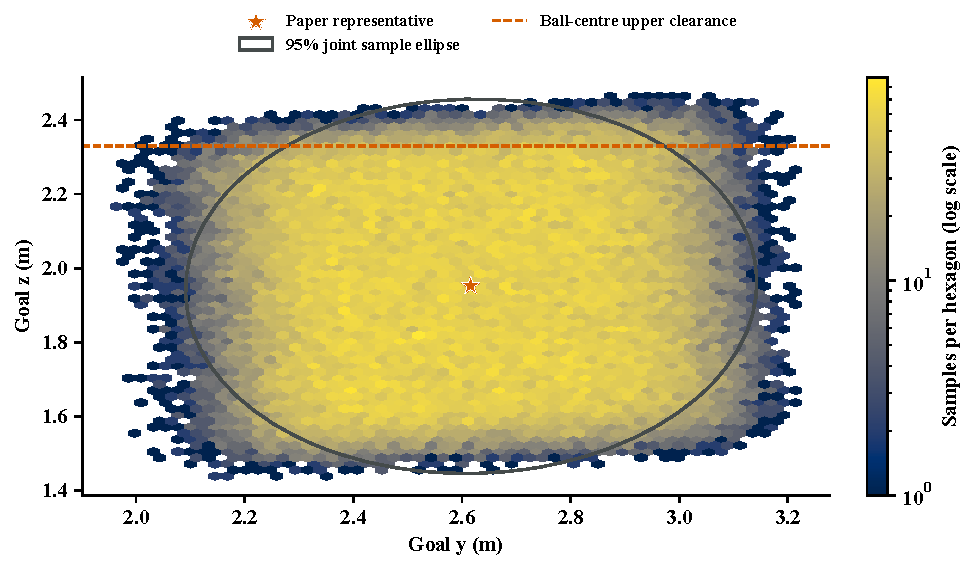
\includegraphics[clip,width=\textwidth]{monte_carlo_crossings.pdf}
\caption{十万次联合扰动的球门交点。六边形颜色表示样本数，椭圆表示联合 95\% 区域，虚线为球心高度上限 $z_g=2.33$ m。}
\end{figure}


图 15 随机展示其中 400 条轨迹，将九项输入与交点坐标、到达时间连接起来。输入按扰动边界缩放至 0--1，输出按十万条轨迹的样本极值缩放至同一区间。展示样本中，385 条蓝色曲线对应完整通过球门的轨迹，15 条橙色曲线对应过高轨迹；每条曲线都给出一组发射条件、气动参数及其预测结果的对应关系。


\begin{figure}[!htbp]
\centering
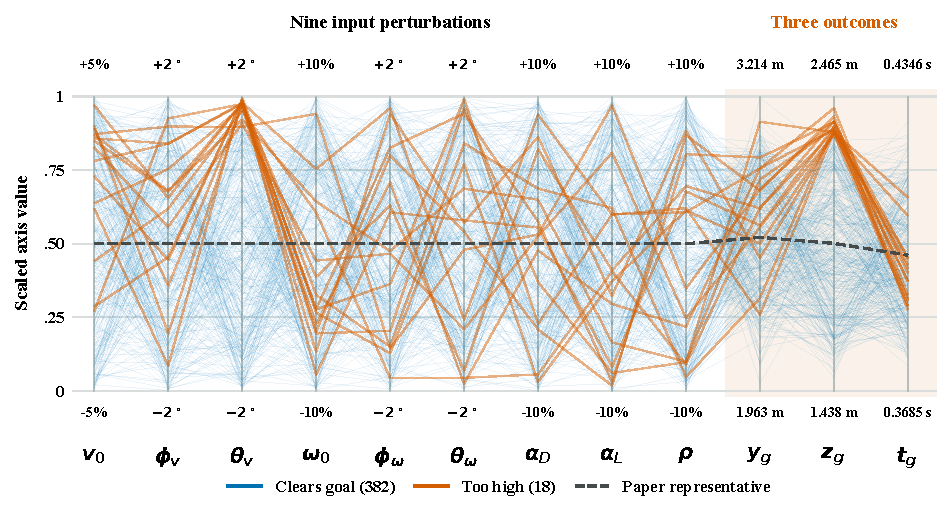
\includegraphics[clip,width=\textwidth]{monte_carlo_parallel_coordinates.pdf}
\caption{输入扰动与球门交点、到达时间的平行坐标图。左侧九轴为输入，右侧三轴为输出；展示样本中有 385 条完整通过球门、15 条过高。}
\end{figure}


图 16 用于检验落点统计结果随模拟次数增加是否趋于稳定，从而判断采用十万次模拟是否足以估计中心 95\% 区间。随着样本增加，蓝色样本极值会因新增的极端轨迹而向外扩展，橙色分位区间则逐渐稳定，反映了两类统计量对样本量的不同响应。当样本量由 50000 增至 100000 时，横向、高度中心 95\% 区间端点的变化分别不超过 0.264 mm、0.506 mm，到达时间区间端点的变化不超过 0.138 ms。另用两个独立随机种子各生成 10000 条轨迹，相应区间端点与主样本的最大差分别为横向 5.425 mm、高度 4.320 mm、时间 0.328 ms。这些比较表明，增加样本对中心区间估计的影响已较小。


\begin{figure}[!htbp]
\centering
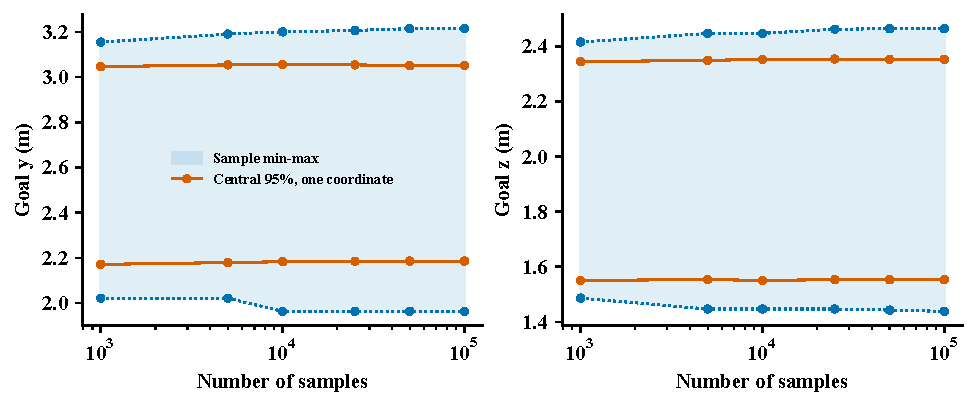
\includegraphics[clip,width=\textwidth]{monte_carlo_convergence.pdf}
\caption{模拟样本量与落点统计量的收敛。蓝色阴影及点线为样本极值，橙色曲线为各坐标的中心 95\% 区间，用于观察区间估计随样本量增加的稳定程度。}
\end{figure}

\FloatBarrier
\end{document}
